\documentclass[10pt,conference]{IEEEtran}
\IEEEoverridecommandlockouts

\usepackage{cite}
\usepackage{amsmath,amssymb,amsfonts}
\usepackage{algorithm}
\usepackage{algpseudocode}
\usepackage{graphicx}
\usepackage{booktabs}
\usepackage{multirow}
\usepackage{array}
\usepackage{textcomp}
\usepackage{xcolor}
\usepackage{url}
\usepackage[hidelinks]{hyperref}

\providecommand{\Description}[1]{}

\newcolumntype{R}[1]{>{\raggedleft\arraybackslash}p{#1}}
\newcommand{\eps}{\varepsilon}
\setcounter{secnumdepth}{3}

\begin{document}

\title{Recalibrating Visual GEO: An Anchor-Decoupled Evaluation Protocol and a Cross-Encoder Transfer Probe on ESCI}

\author{\IEEEauthorblockN{Anonymous Author(s)}
\IEEEauthorblockA{Submission under triple-blind review\\
ICDM 2026}
\thanks{Code, the ESCI manifest, the no-model admissibility verifier, the reference rank-lift scorer, reference implementations of both attacks, reference result tables, and the full reproduction configuration (sampling, seeds, hyper-parameters, hardware) are released anonymously as \textsc{HonestVGEO}: \url{https://anonymous.4open.science/r/honestvgeo-F663}.}}

\maketitle

% tighten float-to-text and displayed-equation spacing to meet the page budget (content-preserving)
\setlength{\textfloatsep}{3.6pt plus 2pt minus 2pt}
\setlength{\dbltextfloatsep}{3.6pt plus 2pt minus 2pt}
\setlength{\floatsep}{4pt plus 2pt minus 2pt}
\setlength{\intextsep}{5pt plus 2pt minus 2pt}
\setlength{\abovedisplayskip}{4pt plus 1pt minus 1pt}
\setlength{\belowdisplayskip}{4pt plus 1pt minus 1pt}
\setlength{\abovedisplayshortskip}{2pt plus 1pt}
\setlength{\belowdisplayshortskip}{2pt plus 1pt}

\begin{abstract}
Visual generative engine optimization edits a product image so it ranks higher under a CLIP-style retriever, and headline results report large cosine-similarity gains at high SSIM, arguing that visual GEO is a serious retrieval-marketplace threat. We show much of this is an artifact of anchor-coupled measurement: when the evaluation query is itself derived from the optimization anchor, any such cosine gain is structurally inflated, shrinking to a bounded, cohort-specific effect under controlled decoupling. We make two contributions to honest threat measurement. First, an anchor-decoupled evaluation protocol --- pinned by a single anchor$\perp$query invariant ($v_{\mathrm{anchor}}(x_p)$ depends only on $x_p$), a pre-flight retriever-discrimination gate, a per-cohort decomposition over the four ESCI human-graded relevance classes, and a compact reference verifier (released as \textsc{HonestEval}) --- that re-measures, rather than amplifies, the white-box threat of our per-image attack CoGEO against three baselines. Second, AE-CoGEO, a query-free, anchor-decoupled cross-encoder transfer \emph{probe} for visual GEO. Its ensemble objective is standard; under the query-free/anchor-decoupled/retrieval-rank constraint triple it yields a calibrated transfer ceiling with a monotone source-count scaling law ($\rho{=}1.0$). On OpenAI ViT-L/14, our CoGEO is the strongest of the four attacks and the unique top-$1$ on five of six retrievers, its white-box advantage concentrated in the harder cohorts and the aggregate mean ($+19.86$, paired Wilcoxon $p \leq 1.1 \times 10^{-4}$, $560$-pair intersection); the per-pair effect is right-skewed (median ${\approx}1$), a cohort-driven, tail-concentrated mean rather than a uniform shift. It trades off monotonically with stealth, and its perturbation transfers far below the white-box ceiling. Properly measured, visual GEO is a cohort-specific, white-box-bounded, transfer-limited, and detectable (AUROC $\geq 0.99$) operator, not a uniform invisible threat.

\end{abstract}

\begin{IEEEkeywords}
visual retrieval, CLIP, adversarial perturbation, generative engine optimization, Amazon ESCI, multimodal evaluation
\end{IEEEkeywords}

\section{Introduction}
\label{sec:intro}

Visual generative engine optimization (VGEO) is the seller-side analogue of search-engine optimization for retrieval systems that match natural-language queries to product images through a shared multimodal embedding~\cite{radford2021clip,aggarwal2023geo}. Imperceptible perturbations of a product image can substantially change its rank under a CLIP-style retriever~\cite{goodfellow2015fgsm,zhou2023advclip,zhang2022coattack}, and headline results report large positive $\Delta$ in cosine similarity together with high SSIM~\cite{wang2004ssim}, arguing that visual GEO is a real threat to retrieval marketplaces.

The conventional evaluation protocol for visual GEO is unsound in a reproducible way: the eval-time query is derived from the same anchor that drove the optimization. When $v_{\mathrm{anchor}}(x_p)$ is the CLIP encoding of a description of $x_p$ and the eval-time similarity is measured against the same caption, any positive $\Delta$ is a tautology of gradient ascent: a measure of optimization vigor, not of retrieval impact under a real shopper query. The eval-time query must therefore be \emph{decoupled} from the optimization anchor.

We deliver \emph{HonestVGEO}, a reusable anchor-decoupled protocol that recalibrates visual GEO into an actionable, defender-relevant threat characterization rather than a deflated headline number. Figure~\ref{fig:framework} sketches the pipeline: a seller-side anchor depending only on $x_p$ feeds four white-box attack families, while a held-out ESCI shopper query enters only at evaluation and never crosses the optimization gradient. The protocol pins three commitments: an \emph{anchor$\perp$query invariant} making the anchor a function of the product image alone, checked by a compact $\sim$60-line reference verifier (released artifact); an \emph{ESCI-grounded benchmark}~\cite{reddy2022esci} of $491$ product images balanced across the four ESCI classes (Exact, Substitute, Complement, Irrelevant) with $560$ paired triples, replicated across six CLIP backbones; and a \emph{four-way comparison} of CoGEO, PGD-bare~\cite{madry2018pgd}, AdvCLIP~\cite{zhou2023advclip}, and Co-Attack~\cite{zhang2022coattack} at $\eps = 16/255$, with per-cohort decomposition and a paired Wilcoxon matrix~\cite{wilcoxon1945individual}. To reach the second, deployment-realistic transfer axis the white-box protocol cannot, we contribute \emph{AE-CoGEO} (\S\ref{sec:method:aecogeo}), the first query-free, anchor-decoupled cross-encoder transfer probe: it optimizes one perturbation against a source-encoder consensus to generalize to an unseen deployed encoder, giving defenders a concrete operator to measure against.

Three claims survive the protocol. \textbf{(C1)} Under the anchor-decoupled protocol, CoGEO is the strongest of the four compared CLIP-targeted attacks on the white-box axis: $+19.86$ mean rank-lift on the four-way intersection, with paired Wilcoxon $p \leq 1.1 \times 10^{-4}$ against every alternative (an aggregate-mean effect carried by the harder cohorts, not a uniform per-pair win over PGD-bare; \S\ref{sec:analysis:exact}) --- not a state-of-the-art claim. \textbf{(C2)} Aggregate dominance hides per-cohort heterogeneity: CoGEO leads by large margins on Complement ($+36.8$) and Irrelevant ($+25.4$); on the Exact cohort the mean rank-lift gap reverses ($+3.9$ for CoGEO vs.\ $+7.1$ for PGD-bare), but matched-pair Wilcoxon and sign tests do not reject the null, so the two methods are statistically balanced rather than dominated. Co-Attack additionally turns negative on Complement, so single-number visual-GEO benchmarks conceal the per-cohort operating regime. \textbf{(C3)} Visual stealth and retrieval lift trade off across attack families: the SSIM means rank in broadly the reverse order from rank-lift (AdvCLIP $0.78 >$ PGD-bare/Co-Attack $0.76 >$ CoGEO $0.66$), and CoGEO's $\mathrm{SSIM} \geq 0.98$ holds at $800 \times 800$ but not at the $224 \times 224$ regime that industrial CLIP retrieval consumes~\cite{radford2021clip}.

The boundary against prior work is twofold. On the evaluation side, any visual-GEO author can run the verifier of \S\ref{sec:method:invariant} before reporting rank-lift, and the multi-method, multi-backbone replication~\cite{cherti2023reproducible,fang2023eva02,zhai2023siglip} establishes the per-cohort pattern as a property of the attack family, not any single embedding. On the attack side, AE-CoGEO is, to our knowledge, the first query-free, anchor-decoupled, cross-encoder-consensus transfer attack for visual GEO (Table~\ref{tab:novelty}). We assume a seller-side attacker with read access to one or more \emph{publicly available} CLIP encoders and unlimited per-image gradient compute, lifting an uploaded perturbation's rank against held-out shopper queries on the same encoder (white-box axis) or an unseen, privately deployed one (transfer axis). A full defensive characterization is beyond our scope, but the transfer measurement (\S\ref{sec:analysis:transfer}) and a training-free detector already characterize visual GEO as a cohort-specific, white-box-bounded, transfer-limited operator.

\section{Related Work}
\label{sec:related}

\paragraph{Generative engine optimization} Generative engine optimization was introduced for text-only generative search engines~\cite{aggarwal2023geo}, where small content edits change which sources a system cites, sharing roots with SEO and adversarial information retrieval~\cite{papernot2017transferable}. Visual GEO extends it to product retrieval ranked by a multimodal embedding rather than a generative LM~\cite{radford2021clip,jia2021scaling}. Our CoGEO attack combines a VLM-derived anchor, a Sobel mask, a differentiable JPEG layer~\cite{shin2017diffjpeg}, and an MI-FGSM loop~\cite{dong2018mifgsm}; it is one of four compared methods, with a VLM captioner~\cite{li2022blip,wang2024qwen2vl} supplying the decoupled anchor text.

\paragraph{CLIP-targeted adversarial attacks} Universal adversarial patches~\cite{zhou2023advclip,moosavidezfooli2017uap} on a CLIP image encoder shift retrieval across diverse inputs, and a complementary family attacks both image and text branches with alternating updates~\cite{zhang2022coattack}; both are query-agnostic, matching the seller-side regime where uploads outpace per-image budgets. The per-image branch descends from PGD~\cite{madry2018pgd} and FGSM~\cite{goodfellow2015fgsm} with momentum~\cite{dong2018mifgsm}, and recent work maps the vulnerability surface of contrastive pretraining~\cite{ilyas2019features,carlini2017cw} and robust-CLIP defenses~\cite{schlarmann2024robustclip}. What is missing is evaluation under held-out human relevance: prior work scores against queries derived from the optimization signal itself, never a multi-cohort benchmark with a published anchor$\perp$query invariant.

\paragraph{Transfer-based attacks and cross-encoder consensus} A long line improves the black-box transferability of per-image attacks through input-diversity~\cite{xie2019dim} and scale-invariant~\cite{lin2020sim} transformations, momentum~\cite{dong2018mifgsm}, and optimization against an ensemble of surrogate models~\cite{papernot2017transferable}, so a perturbation crafted on accessible models survives on an unseen one. These techniques were developed for image classification and still presume a target label or a query/caption at attack time~\cite{zhang2022coattack}. AE-CoGEO (\S\ref{sec:method:aecogeo}) is, to our knowledge, the first to bring ensemble-consensus transfer to visual GEO under the query-free, anchor-decoupled constraint, measuring rank-lift on held-out encoders that never entered the optimization set (\S\ref{sec:analysis:transfer}). Table~\ref{tab:novelty} positions it among these families.

\begin{table}[t]
\centering
\scriptsize
\setlength{\tabcolsep}{4pt}
\caption{Where AE-CoGEO sits among adversarial attacks on the four axes visual GEO imposes. \textbf{QF}: query/caption-free attack; \textbf{HE}: scored under held-out human relevance (anchor$\perp$query); \textbf{XE}: transfers to an unseen encoder via source-set consensus; \textbf{VG}: optimizes retrieval rank, not classification. AE-CoGEO uniquely satisfies all four; \textbf{HE} holds only for our protocol.}
\label{tab:novelty}
\begin{tabular}{@{}lcccc@{}}
\toprule
Attack & QF & HE & XE & VG \\
\midrule
PGD / FGSM~\cite{madry2018pgd,goodfellow2015fgsm} & \checkmark & $\times$ & $\times$ & $\times$ \\
MI/DI/SI-FGSM~\cite{dong2018mifgsm,xie2019dim,lin2020sim} & \checkmark & $\times$ & $\times$ & $\times$ \\
Ensemble transfer~\cite{papernot2017transferable} & \checkmark & $\times$ & \checkmark & $\times$ \\
AdvCLIP patch~\cite{zhou2023advclip} & \checkmark & $\times$ & $\times$ & \checkmark \\
Co-Attack~\cite{zhang2022coattack} & $\times$ & $\times$ & $\times$ & \checkmark \\
CoGEO (ours) & \checkmark & \checkmark & $\times$ & \checkmark \\
\textbf{AE-CoGEO (ours)} & \checkmark & \checkmark & \checkmark & \checkmark \\
\bottomrule
\end{tabular}
\end{table}

\paragraph{Held-out relevance evaluation} The Amazon ESCI dataset~\cite{reddy2022esci} provides $(q, x_p, \ell)$ triples with four-class human labels (Exact, Substitute, Complement, Irrelevant), and to our knowledge has not previously been used to evaluate adversarial image perturbations; we add a Food-101~\cite{bossard2014food101} consistency check. Because ESCI queries come from real shoppers and labels are independent of any retriever's geometry, observed rank-lift measures something other than the gradient that produced it, placing the protocol in the held-out tradition of BEIR~\cite{thakur2021beir} and MTEB~\cite{muennighoff2023mteb} that rejects self-loop similarity~\cite{schlarmann2024robustclip,mao2023zsar}. Per-cohort decomposition is a first-class output, not a post-hoc breakdown.

\paragraph{Stealth and replication} SSIM~\cite{wang2004ssim} is the canonical perceptual-quality measure, but visual-GEO stealth claims are often reported at the optimization resolution ($800{\times}800$) rather than the $224{\times}224$ input the retriever consumes --- a discrepancy not previously characterized across attack families on one benchmark. We report the four-method stealth--lift Pareto at native input size and replicate across six CLIP backbones~\cite{radford2021clip,cherti2023reproducible,fang2023eva02,zhai2023siglip}, separating embedding-specific dominance from dominance over per-image gradient attacks across CLIP-style embeddings.

\section{Anchor-Decoupled Evaluation Protocol}
\label{sec:method}


\begin{figure*}[t]
\centering
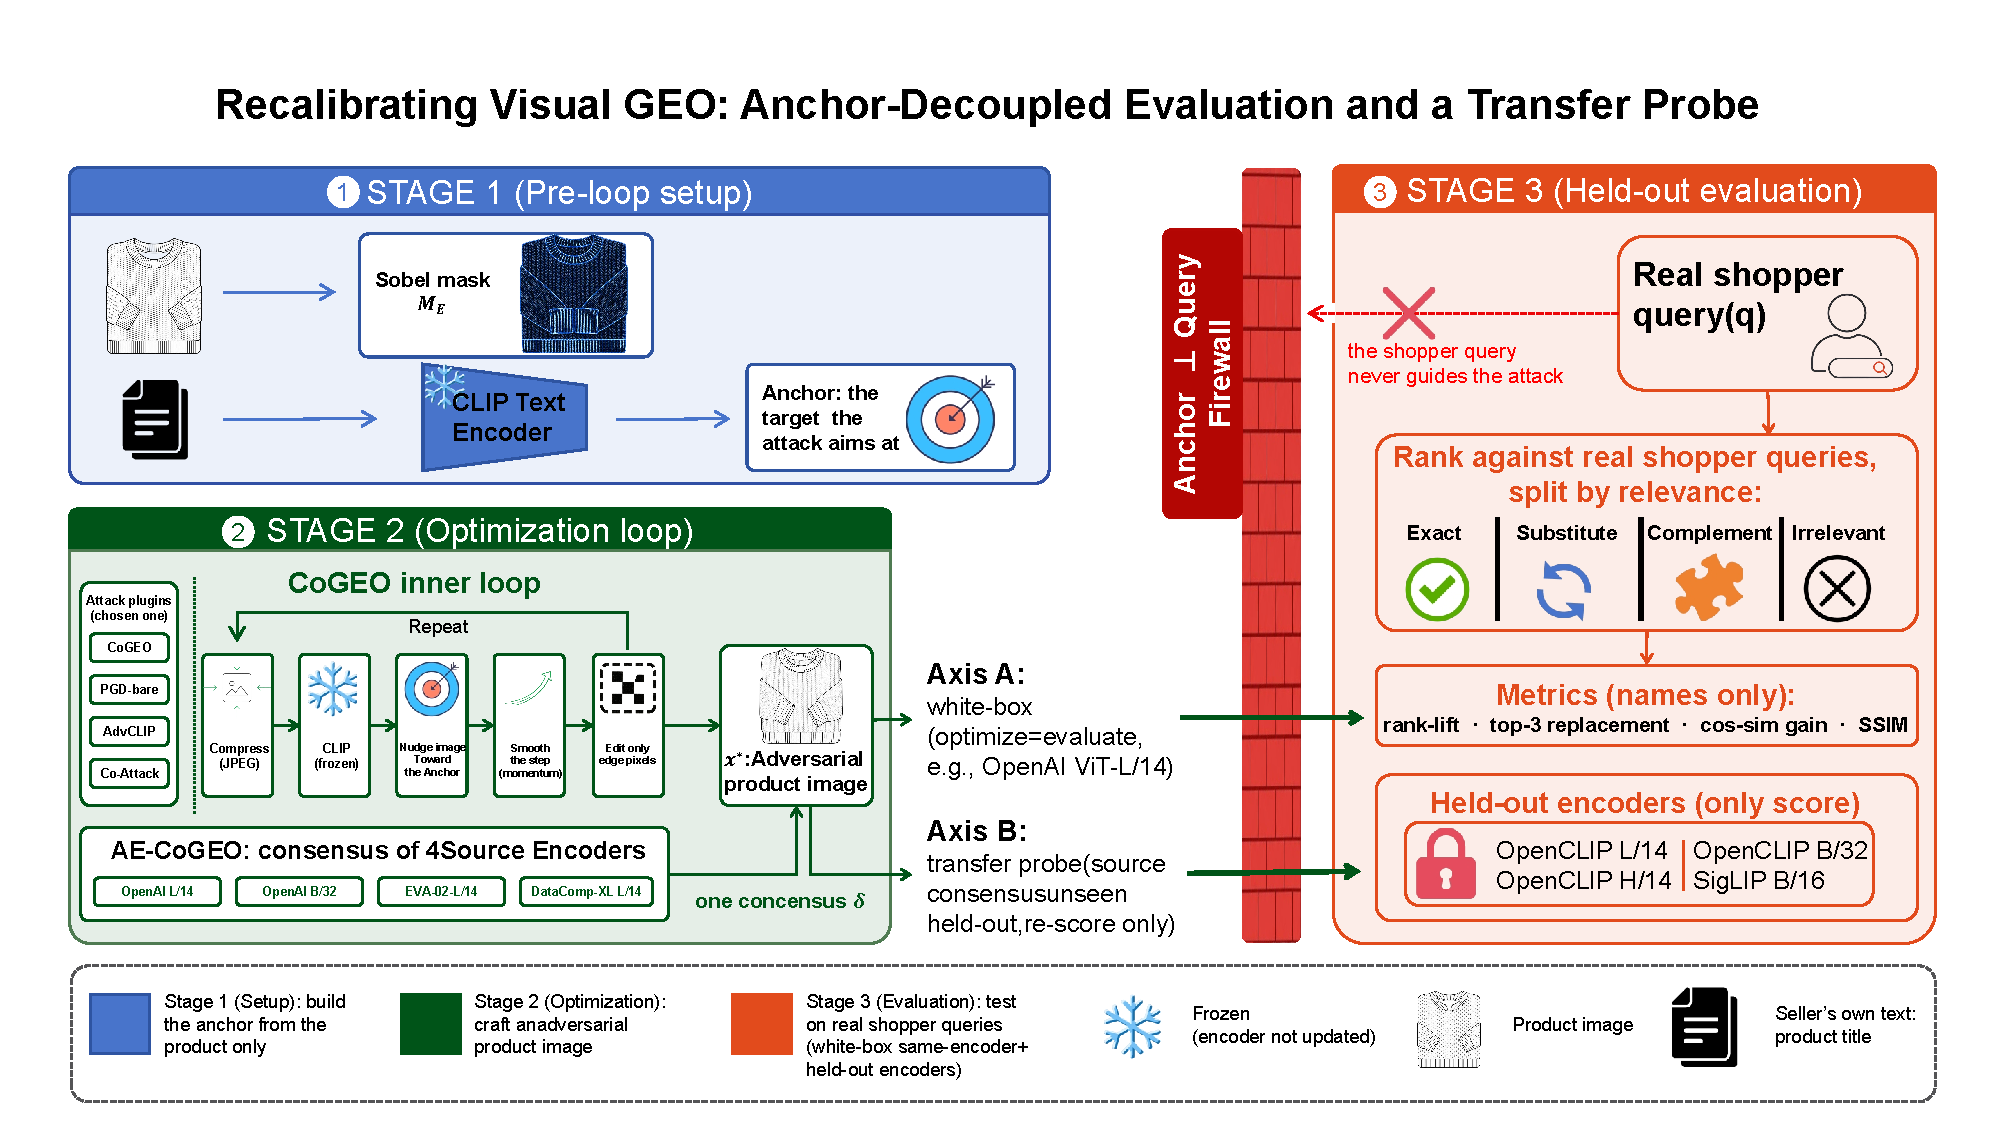
\includegraphics[width=0.85\textwidth]{figures/fig_framework.pdf}
\caption{Anchor-decoupled evaluation protocol with a cross-encoder transfer probe, instantiated for CoGEO. \textbf{Stage~1} precomputes the seller anchor $v_{\mathrm{anchor}}{=}E_T(t_p^{\star})$ from the product title and a Sobel-edge mask $M_E$ (top-$40\%$ gradient pixels); $v_{\mathrm{anchor}}$ depends on the product image alone, never on a shopper query. \textbf{Stage~2} runs the CoGEO inner loop---JPEG-compress, encode with the frozen CLIP tower, nudge toward the anchor, smooth with momentum, edit only masked edge pixels---for $K{=}200$ iterations at $\varepsilon{=}16/255$; baselines PGD-bare, AdvCLIP and Co-Attack drop or replace individual boxes. Two orthogonal axes, not competing attacks: \emph{Axis~A} optimizes against a single white-box encoder; \emph{Axis~B} (AE-CoGEO) against a four-source consensus loss $L_{\mathrm{ens}}{=}-\tfrac{1}{|\mathcal{S}|}\sum_{j}\cos(E_I^{(j)}(\tilde{x}),E_T^{(j)}(t_p^{\star}))$. \textbf{Stage~3} scores the frozen image against unseen ESCI shopper queries across the four cohorts (E/S/C/I) and re-scores Axis~B---no re-attack---on four held-out encoders. The shopper query never crosses the Anchor-Decoupled Query Firewall. Snowflakes mark frozen modules.}
\Description{Three-stage anchor-decoupled pipeline with a transfer probe. Stage one builds a frozen text anchor from the product title together with a Sobel gradient mask; the anchor depends only on the product image, never on the shopper query. Stage two runs a five-step perturbation loop (differentiable JPEG, frozen image encoding, anchor-alignment cosine loss, momentum gradient, masked projection) and splits into two orthogonal axes: a white-box axis against a single encoder, and a transfer axis (AE-CoGEO) that optimizes a four-encoder consensus loss over optimize-only source encoders. Stage three scores the frozen image against unseen shopper queries across four relevance cohorts and re-scores the transfer axis on four held-out encoders without re-attacking; the query is separated from the optimization path by an anchor-decoupled query firewall.}
\label{fig:framework}
\end{figure*}

\subsection{\texorpdfstring{The anchor$\perp$query invariant}{The anchor-perpendicular-query invariant}}
\label{sec:method:invariant}

Let $x_p$ denote a product image, $q$ a shopper query in natural language, $E_I$ and $E_T$ the image and text encoders of a CLIP-style retriever~\cite{radford2021clip,jia2021scaling,cherti2023reproducible}, and $v_{\text{anchor}}(x_p) \in \mathbb{R}^d$ a target text embedding used to drive a perturbation $\delta$ such that $E_I(x_p + \delta)$ moves toward $v_{\text{anchor}}(x_p)$.

We require that, for every $(q, x_p)$ pair used in evaluation,
\begin{equation}
v_{\text{anchor}}(x_p)\ \text{is a function of}\ x_p\ \text{alone,}\ \text{not of}\ q.
\label{eq:invariant}
\end{equation}
Concretely, $v_{\text{anchor}}$ may be the CLIP text encoding of the product category, of a VLM description of $x_p$ (varied across BLIP, BLIP-2, LLaVA-1.5, Qwen2-VL, and Qwen2.5-VL in the released artifact), or of the product title; in all cases it depends only on the seller-side description. The query $q$ enters only at evaluation time, when we measure rank-lift, top-3 replacement, and held-out cosine similarity gains under $q$.

This invariant is the operational definition of an honest visual-GEO evaluation: when the eval query is itself derived from $v_{\text{anchor}}$, the similarity gain is structurally inflated relative to held-out retrieval impact. We enforce \eqref{eq:invariant} at the code level across all four families with a compact reference verifier ($\sim$60 lines, released artifact) that statically rejects any query-like attack parameter and dynamically checks that the perturbation is byte-identical across swapped eval queries under a fixed seed.

\subsection{Pre-flight monotonicity gate}
\label{sec:method:noop}

Before any adversarial perturbation, the chosen retriever must demonstrate that human-graded relevance labels are discriminable in its embedding space. Writing $\overline{\cos}_{\ell} = \mathrm{mean}_{(q,x_p)\in\ell}\bigl[\cos(E_I(x_p),\,E_T(q))\bigr]$ for the mean no-perturbation cosine over a cohort $\ell$, we require that on a balanced sample of $(q, x_p, \ell)$ triples spanning the four ESCI relevance classes Exact (E), Substitute (S), Complement (C), Irrelevant (I), the gate
\begin{equation}
\overline{\cos}_{\ell=E} - \overline{\cos}_{\ell=I} \;\geq\; 0.05
\label{eq:noop_gate}
\end{equation}
holds.
A retriever that fails \eqref{eq:noop_gate} cannot serve as an evaluation substrate: no adversarial pressure is measurable against an embedding that cannot already separate Exact-match from Irrelevant pairs. We read $0.05$ as a qualitative admissibility floor, not a calibrated statistic: a conservative margin that the canonical CoGEO retriever (ViT-L/14, gap $0.0533$) clears and a markedly weaker substrate (ViT-B/32, $0.0405$) does not, with both satisfying $E\!>\!S\!>\!C\!>\!I$ monotonicity. The evaluation substrate (ViT-L/14) is fixed independently as the canonical retriever, so no downstream result depends on the exact floor value. On failure, the protocol mandates a backbone swap before optimization.

\subsection{Four-way attack pass}
\label{sec:method:attacks}

Within the invariant, four white-box attack families are evaluated at a matched perturbation budget $\eps = 16/255$, the cross-family normalization point at which all four families separate cleanly (not a claim that it is the only deployment-relevant budget; the budget-dependence is examined in \S\ref{sec:analysis:eps}):

\paragraph{CoGEO} Per-image projected gradient descent~\cite{madry2018pgd,goodfellow2015fgsm} on $x_p$ with momentum (MI-FGSM~\cite{dong2018mifgsm}), Sobel-edge mask restricting perturbation to high-gradient regions, environment simulation through a differentiable JPEG layer~\cite{shin2017diffjpeg} together with input-diversity~\cite{xie2019dim} and scale-invariant~\cite{lin2020sim} transformations, and product-title $v_{\text{anchor}}$; CoGEO is the attack we propose and the primary subject of the held-out evaluation. Adapting it to the anchor-decoupled protocol fixes three design choices, each settled by an ablation in the released artifact: a hard top-$40\%$ Sobel-gradient mask (vs.\ a soft min-max-normalized mask floored at $0.1$), differentiable JPEG at $Q{=}75$ (vs.\ $Q{=}85$), and translation-invariant smoothing omitted, as it gave no significant lift under the anchor$\perp$query setting.

Formally, let $x_p^{(k)}$ denote the listing image at iteration $k$ (with $x_p^{(0)}{=}x_p$). The Sobel edge mask
\begin{equation}
M_E \;=\; \mathbf{1}\!\bigl[\,|\nabla_{\mathrm{Sobel}}\,x_p|\;\geq\;q_{0.6}(|\nabla_{\mathrm{Sobel}}\,x_p|)\,\bigr]
\label{eq:sobel_mask}
\end{equation}
selects the top-$40\%$ gradient pixels (threshold $q_{0.6}$, the $60$-th percentile of edge magnitude) and is computed once per image. At each iteration $k$, CoGEO applies a differentiable JPEG layer at quality $Q{=}75$ to make the attack compression-aware, embeds the result with the frozen CLIP image encoder, and forms the anchor-alignment loss
\begin{equation}
L^{(k)} \;=\; -\,\cos\!\bigl(\,E_I(\mathrm{diffJPEG}_{Q=75}(x_p^{(k)})),\; v_{\mathrm{anchor}}\,\bigr).
\label{eq:anchor_loss}
\end{equation}
The signed gradient is smoothed by a momentum buffer with $\mu=1.0$ following the original MI-FGSM formulation~\cite{dong2018mifgsm}:
\begin{equation}
g^{(k+1)} \;=\; \mu\,g^{(k)} \;+\; \frac{\nabla_{x}\,L^{(k)}}{\lVert\nabla_{x}\,L^{(k)}\rVert_1}, \quad \mu = 1.0,
\label{eq:mifgsm_momentum}
\end{equation}
The masked signed-momentum step (step size $\alpha = 4/255$) is then projected onto the $\ell_\infty$ $\varepsilon$-ball $\mathcal{B}_\infty(x_p,\varepsilon){=}\{x:\lVert x-x_p\rVert_\infty{\leq}\varepsilon\}$:
\begin{equation}
x_p^{(k+1)} \;=\; \Pi_{\mathcal{B}_\infty(x_p,\,\varepsilon)}\!\Bigl( x_p^{(k)} - \alpha \cdot \mathrm{sign}\bigl(M_E \odot g^{(k+1)}\bigr) \Bigr).
\label{eq:masked_step}
\end{equation}
After $K{=}200$ iterations, $x_p^{\star}$ is the adversarial image evaluated against the held-out query in \S\ref{sec:method:metrics}.

\paragraph{PGD-bare} The same product-title $v_{\text{anchor}}$ as CoGEO but without the Sobel mask, environment simulation, or momentum, recovering the classical signed-step PGD baseline of~\cite{madry2018pgd} and isolating the anchor's contribution from the engineering layered on top.

\paragraph{AdvCLIP} A query-agnostic universal adversarial patch~\cite{moosavidezfooli2017uap,thys2019adversarialpatches} trained on the CLIP image encoder~\cite{zhou2023advclip} over 30 epochs with budget $\eps = 16/255$, applied to each $x_p$ at evaluation. AdvCLIP requires no per-image gradient pass at deployment time.

\paragraph{Co-Attack} A cross-modal alternating attack~\cite{zhang2022coattack} that interleaves an $L_\infty$ image perturbation ($\eps = 16/255$) and an $L_2$ text-anchor perturbation ($\eps_v = 0.1$) over 200 iterations. The text branch operates on the seller-side anchor only, never on $q$, so the invariant is preserved.

All four pipelines take only $x_p$ as optimization input; the held-out ESCI query never enters any optimization gradient, verified at the code level.

The CoGEO inner loop is fully specified by Eqs.~\eqref{eq:sobel_mask}--\eqref{eq:masked_step}; the full evaluation-pass pseudocode is in the released artifact.

\subsection{AE-CoGEO: a cross-encoder-consensus transfer probe}
\label{sec:method:aecogeo}

The four-way comparison above is a \emph{white-box} measurement: the encoder that drives the perturbation also scores it. This bounds one axis --- how far an attacker can move the ranking of a retriever it fully controls --- but leaves unmeasured the realistic deployment axis, where the platform retriever is an \emph{unseen} encoder the attacker never optimized against. We introduce \textbf{AE-CoGEO} (Anchor-decoupled Ensemble CoGEO) to measure this second axis.

AE-CoGEO keeps both protocol commitments of CoGEO unchanged --- the perturbation is \emph{query-free} and \emph{anchor-decoupled}, so the held-out shopper query never enters optimization (\eqref{eq:invariant}) --- and adds a single mechanism: instead of aligning to one encoder, it optimizes one perturbation against the \emph{consensus} of a source set of encoders $\mathcal{S}=\{(E_I^{(j)}, E_T^{(j)})\}_{j=1}^{m}$ ($m=|\mathcal{S}|=4$ source encoders). Writing $t_p^{\star}=\textsc{SellerAnchor}(x_p)$ for the seller-side anchor text and $\tilde{x}=\mathrm{diffJPEG}_{Q}(x_p+\delta)$, the anchor-alignment loss is averaged over the source set,
\begin{equation}
L_{\mathrm{ens}}(\delta) = -\frac{1}{m}\sum_{j=1}^{m} \cos\bigl(E_I^{(j)}(\tilde{x}),\, E_T^{(j)}(t_p^{\star})\bigr),
\label{eq:ens_loss}
\end{equation}
and the masked MI-FGSM update of \eqref{eq:mifgsm_momentum}--\eqref{eq:masked_step} is applied to $\nabla_\delta L_{\mathrm{ens}}$ without change, so $\delta$ raises anchor alignment \emph{simultaneously} across architectures rather than overfitting one encoder's geometry. Ensemble optimization is a standard transferability route~\cite{papernot2017transferable,dong2018mifgsm,xie2019dim}; AE-CoGEO's increment is combining it diagnostically with the query-free, anchor-decoupled constraint visual GEO imposes.

Source and held-out encoders are strictly disjoint: the source set is $\mathcal{S}=\{$OpenAI ViT-L/14, OpenAI ViT-B/32, EVA-02-L/14, DataComp-XL ViT-L/14$\}$ and the held-out set is $\{$OpenCLIP-L/14, -H/14, -B/32 (all LAION-2B), SigLIP ViT-B/16$\}$, with no shared checkpoint and no shared pretraining corpus. Every other setting --- $\eps=16/255$, $K=200$, Sobel mask, differentiable-JPEG and input-diversity environment simulation, and product-title anchor --- is identical to the single-encoder CoGEO arm, so any change in held-out behavior is attributable to the consensus mechanism alone.

CoGEO and AE-CoGEO thus instrument two orthogonal axes of the same threat --- the white-box and transfer ceilings --- with AE-CoGEO the calibrated transfer probe; \S\ref{sec:analysis:transfer} reports the measurement.

\subsection{Per-cohort decomposition and significance}
\label{sec:method:metrics}

For each adversarial image $x_p^* = x_p + \delta$ we compute four metrics against the held-out query~$q$: \emph{rank-lift} $\mathrm{rank}(x_p, q) - \mathrm{rank}(x_p^*, q)$, the positions $x_p^*$ rises for $q$; \emph{top-3 replacement rate}, the fraction of pairs where $x_p^*$ enters the top $3$ while $x_p$ did not; \emph{held-out} $\Delta_{\mathrm{clip\_sim}} = \cos(E_I(x_p^*), E_T(q)) - \cos(E_I(x_p), E_T(q))$, the direct CLIP-similarity gain under $q$; and \emph{SSIM} between $x_p$ and $x_p^*$ at the retriever's native resolution, the stealth at the regime industrial retrieval consumes. Every metric is then \emph{decomposed} per cohort over the four ESCI relevance classes. Aggregate means across all pairs are reported alongside per-cohort means, never as a substitute. We further compute a paired Wilcoxon signed-rank test for each of the $\binom{4}{2}=6$ method pairs on the same $(q, x_p)$ index, so each pairwise comparison is verifiable independently of any cohort selection.


\section{Experimental Setup}
\label{sec:setup}

We instantiate the protocol of Section~\ref{sec:method} on the Amazon ESCI shopper-query benchmark and run all four attack families against the same set of product images.

\subsection{Benchmark and sampling}
\label{sec:setup:bench}

We sample $(q, x_p, \ell)$ triples from the Amazon ESCI dataset~\cite{reddy2022esci} (US locale), with $\ell \in \{E, S, C, I\}$ a four-level human-graded relevance label authored by real shoppers and independent of any retriever embedding. A label-balanced sample (random seed $42$) yields $491$ unique product images and $560$ paired triples --- $125$ Exact, $125$ Substitute, $185$ Complement, $125$ Irrelevant --- each resized to $224 \times 224$~\cite{radford2021clip} (CDN resolution in the released artifact). We additionally replicate the protocol on Food-101~\cite{bossard2014food101} as a ranking-internal-consistency check (Fig.~\ref{fig:results}f); because its cohorts are CLIP-text-similarity quartiles over the $101$ class names, they are retriever-induced and not promoted to ESCI-equivalent human-graded relevance evidence.

\subsection{Retriever and budgets}
\label{sec:setup:budget}

The retriever is OpenAI CLIP ViT-L/14~\cite{radford2021clip} used identically as both the optimization target and the evaluation embedder, fixed a priori as the canonical CoGEO retriever; it also clears the pre-flight gate of \eqref{eq:noop_gate} ($\mathrm{gap}_{E-I} = 0.0533 > 0.05$), whereas a weaker ViT-B/32 ($0.0405$) would not (full backbone sensitivity table in the released artifact). Cross-backbone replication uses five additional CLIP-style retrievers from the OpenCLIP toolbox~\cite{cherti2023reproducible} that vary pretraining corpus and architecture: OpenCLIP-L/14 (LAION-2B), EVA-02-L/14~\cite{fang2023eva02}, SigLIP ViT-B/16~\cite{zhai2023siglip}, OpenCLIP ViT-B/32, and OpenCLIP ViT-H/14. Anchor-source robustness is measured separately in the released artifact using five VLM captioner anchors --- BLIP~\cite{li2022blip}, BLIP-2~\cite{li2023blip2}, LLaVA-1.5~\cite{liu2024llava}, Qwen2-VL~\cite{wang2024qwen2vl}, Qwen2.5-VL~\cite{bai2024qwen25vl} --- over the same six backbones ($30$ CoGEO cells).

For each held-out query $q_i$, rank-lift is computed against a fixed per-query candidate pool of size $C{=}491$ (the union of all manifest ASIN images), making it a within-pool diagnostic over the $491$-image manifest rather than an absolute marketplace-scale rank: \emph{rank} is the position of $x_{p,i}^{\star}$ in the descending $\cos(E_I(\cdot),\,E_T(q_i))$ sort. All four families operate at matched $\eps = 16/255$ in $L_\infty$, with $\eps \in \{4, 8\}/255$ sweeps in Fig.~\ref{fig:results}b. CoGEO and PGD-bare run $T = 200$ momentum signed-step PGD iterations~\cite{madry2018pgd,dong2018mifgsm}; CoGEO adds a differentiable JPEG layer~\cite{shin2017diffjpeg} and input-diversity transforms~\cite{xie2019dim,lin2020sim}. AdvCLIP trains its universal patch~\cite{moosavidezfooli2017uap,thys2019adversarialpatches,zhou2023advclip} over the same manifest used at evaluation, a regime favorable to AdvCLIP, so CoGEO's dominance is conservative. Co-Attack runs $200$ alternating iterations at image $\eps = 16/255$, text $\eps_v = 0.1$~\cite{zhang2022coattack}, its text branch perturbing a fixed seller-side anchor (\emph{not} the held-out query). Anchor sources are held constant within method (product-title for CoGEO/PGD-bare, image-only for AdvCLIP; full hyper-parameters in the released artifact).

\subsection{Significance protocol}

For each comparison we report the paired Wilcoxon signed-rank test~\cite{wilcoxon1945individual} on rank-lift, paired bootstrap $95\%$ CIs (1000 resamples), and the held-out $\Delta_{\mathrm{clip\_sim}}$ mean; SSIM~\cite{wang2004ssim} is reported at the native $224\times 224$ input. Directional tests are one-sided; the six pairwise $p$-values are reported uncorrected, but the headline comparisons survive Holm--Bonferroni at the six-test count (the strongest, $p = 3.5 \times 10^{-30}$, survives any correction). The full $4 \times 4$ matrix is in the released artifact (\S\ref{sec:analysis:wilcoxon}).

\section{Main Results}
\label{sec:experiments}

Table~\ref{tab:main4way} reports the headline four-way comparison on the full $560$-pair intersection. These results measure the \emph{white-box axis}, where optimization and scoring encoders coincide; the deployment-realistic \emph{transfer axis} (AE-CoGEO, \S\ref{sec:method:aecogeo}) is measured separately in \S\ref{sec:analysis:transfer}. Three findings emerge.

\begin{table}[htbp]
\centering
\caption{Four-way comparison on the $560$-pair joint sample at $\eps = 16/255$ with CLIP ViT-L/14. Rank-lift is the mean positions an image rises against its held-out ESCI query; SSIM is at the $224 \times 224$ input; $p$-values are one-sided paired Wilcoxon versus CoGEO; I$\to$top-3 gain is against the unperturbed baseline.}
\label{tab:main4way}
\small
\begin{tabular}{lrrrr}
\toprule
Method     & Rank-lift & $p$ vs CoGEO & SSIM  & I$\to$top-3 gain \\
\midrule
CoGEO      & \textbf{19.86} & ---            & 0.66  & \textbf{+4.1\,pp} \\
PGD-bare   & 12.37          & $1.1 \times 10^{-4}$ & 0.76  & +2.9\,pp \\
AdvCLIP    & ~6.45          & $3.5 \times 10^{-30}$ & \textbf{0.78} & +1.6\,pp \\
Co-Attack  & ~5.77          & $1.3 \times 10^{-8}$  & 0.76  & +2.9\,pp \\
\bottomrule
\end{tabular}
\end{table}

\paragraph{Aggregate-mean dominance is significant} CoGEO's $+19.86$ mean rank-lift is $1.6\times$ the next-best baseline, with every pairwise paired Wilcoxon $p$-value well below $0.05$ (to $3.5 \times 10^{-30}$ versus AdvCLIP); the four-way intersection sharpens significance by including pairs on which AdvCLIP and Co-Attack both fail to move the ranking. AdvCLIP's universal patch~\cite{zhou2023advclip} moves the ranking least --- a single $\delta$ against a fixed text concept does not adapt to per-image content~\cite{moosavidezfooli2017uap} --- and Co-Attack is statistically below PGD-bare ($p = 2.4 \times 10^{-6}$); its text-anchor branch does not compensate for the loss of CoGEO's mask and momentum~\cite{dong2018mifgsm,xie2019dim,lin2020sim}.

\paragraph{Visual stealth and retrieval lift trade off} The four SSIM values~\cite{wang2004ssim} rank in the opposite order from rank-lift (Table~\ref{tab:main4way}): at $800 \times 800$ CoGEO's $\mathrm{SSIM}$ is $\geq 0.98$, but at the $224 \times 224$ regime the retriever consumes all four fall to low SSIM (CoGEO $0.66$, stealthiest AdvCLIP $0.78$; Section~\ref{sec:analysis:ssim}). The right-most column of Table~\ref{tab:main4way} reports the metric a defender ultimately cares about --- pushing Irrelevant products into the top-3 a shopper sees, against a $9.1\%$ unperturbed baseline --- where CoGEO translates its largest aggregate lift into top-3 placement.

\section{Analysis}
\label{sec:analysis}

The aggregate result of \S\ref{sec:experiments} hides a structurally heterogeneous picture, decomposed below along cohort, pairwise significance, stealth, perturbation-budget sensitivity, the Exact-cohort failure mode, cross-backbone replication, transfer, and anchor robustness, then consolidated under a bounded-under-stress synthesis (further replications in the released artifact).

\begin{figure*}[t]
\centering
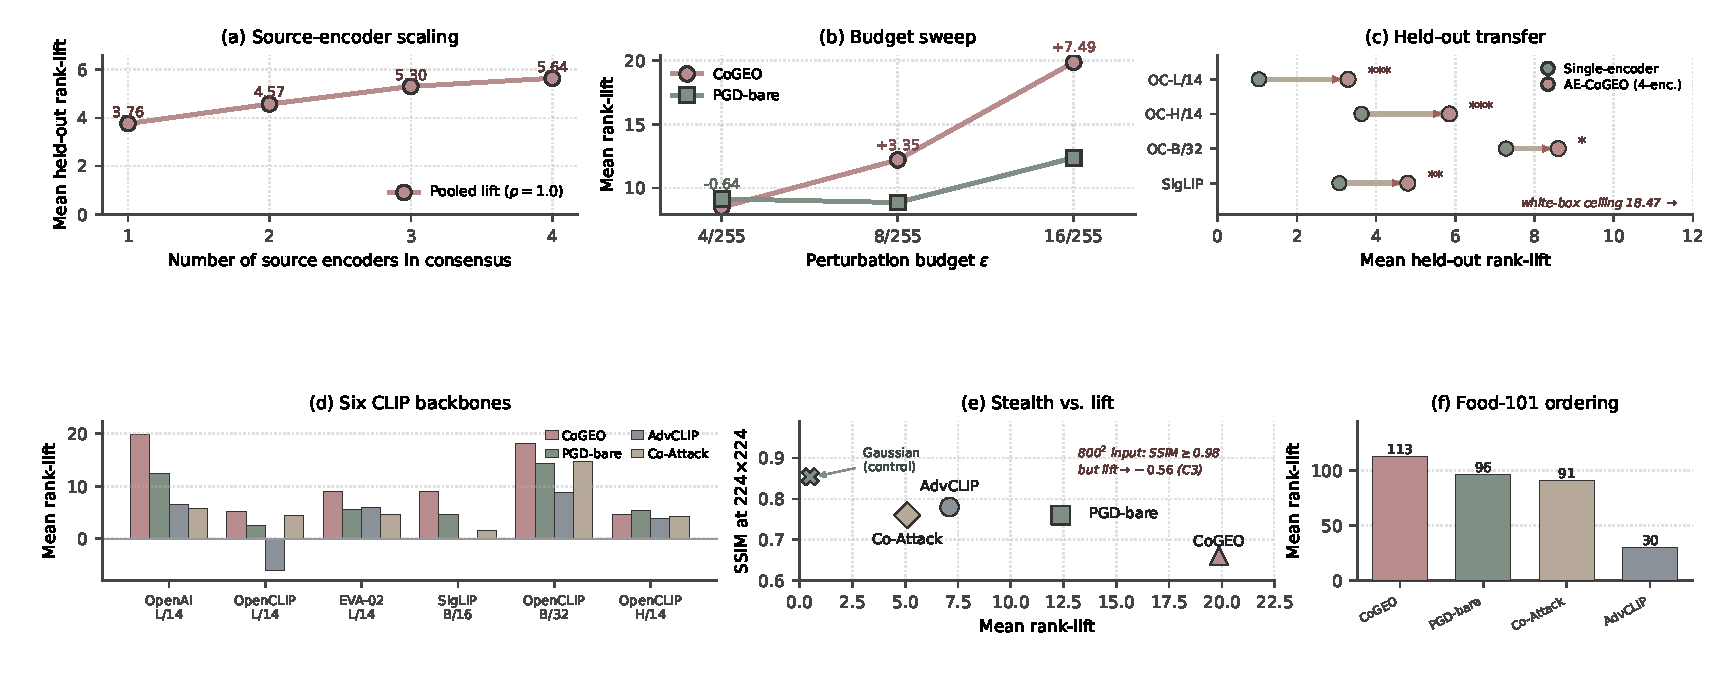
\includegraphics[width=\textwidth]{figures/fig_results_main.pdf}
\caption{AE-CoGEO transfer behavior and protocol robustness; every value matches a manuscript table. \textbf{(a)} Rank-lift scales with the source-encoder count ($3.76\to5.64$, $\rho=1.0$). \textbf{(b)} Budget sweep (OpenAI ViT-L/14): the CoGEO$-$PGD-bare margin inverts at $\eps=4/255$ ($-0.64$) and grows to $+7.49$ at $16/255$. \textbf{(c)} Held-out transfer (single-encoder~$\to$~four-encoder consensus, $n=498$, Table~\ref{tab:transfer}): the consensus lifts all four unseen encoders (one-sided paired Wilcoxon; $^{*}p<5\!\times\!10^{-2}$, $^{**}p<10^{-2}$, $^{***}p<10^{-3}$) but stays below the white-box ceiling (dashed). \textbf{(d)} Four-way rank-lift across six CLIP backbones ($\eps=16/255$): CoGEO is the unique top-1 on five of six. \textbf{(e)} Stealth/lift trade-off (Table~\ref{tab:main4way}): higher rank-lift costs SSIM, all below high fidelity at $224\times224$ (CoGEO $0.66$, AdvCLIP $0.78$). \textbf{(f)} Food-101 cross-dataset check ($505$ triples, OpenAI ViT-L/14): the ESCI ordering CoGEO $>$ PGD-bare $>$ Co-Attack $>$ AdvCLIP is preserved (gap $1.61\times\!\to\!1.17\times$).}
\label{fig:results}
\end{figure*}

\subsection{Per-cohort rank-lift decomposition}
\label{sec:analysis:cohort}

\begin{table}[t]
\centering
\caption{Per-cohort mean rank-lift over the four ESCI relevance classes ($560$-pair, OpenAI ViT-L/14, $\eps=16/255$): the per-cohort heterogeneity claim \textbf{(C2)}. Bold marks the per-cohort best; sizes $n=125$ for E/S/I and $185$ for C; values match Table~\ref{tab:main4way}.}
\label{tab:cohort}
\small
\setlength{\tabcolsep}{5pt}
\begin{tabular}{lrrrr}
\toprule
Method & Exact & Substitute & Complement & Irrelevant \\
 & ($n{=}125$) & ($n{=}125$) & ($n{=}185$) & ($n{=}125$) \\
\midrule
CoGEO     & 3.90 & 5.24 & \textbf{36.77} & \textbf{25.43} \\
PGD-bare  & \textbf{7.12} & 1.84 & 18.86 & 18.53 \\
AdvCLIP   & 1.00 & 0.94 & 14.46 & 5.53 \\
Co-Attack & 6.18 & \textbf{5.47} & $-1.86$ & 16.94 \\
\bottomrule
\end{tabular}
\end{table}

Table~\ref{tab:cohort} reports the same rank-lift quantity as Table~\ref{tab:main4way}, split across the four ESCI cohorts (sizes $n=125$ for E/S/I and $185$ for C); the split materially reshapes the headline.

Three patterns emerge. First, CoGEO's dominance is not uniform: on Exact, PGD-bare's mean exceeds CoGEO's by $\sim3.2$ positions, yet matched-pair tests find no systematic per-pair advantage, so PGD-bare only \emph{approximately matches} CoGEO there (\S\ref{sec:analysis:exact}). Second, Complement is where CoGEO's machinery yields its largest gain ($+36.8$, $1.95\times$ PGD-bare; a small-sample peak that resolves to strict $E\!<\!S\!<\!C\!<\!I$ at $3\times$ scale, \S\ref{sec:analysis:summary}). Third, Co-Attack alone turns negative on Complement ($-1.86$), its alternating image--text branch degrading ranking when the image--text correlation is already weak. The aggregate ranking thus conceals a method-specific regime: \emph{visual GEO is a cohort-specific operator} whose lift concentrates on the harder, lower-relevance cohorts (peaking on Complement, strong on Irrelevant) while gaining no per-pair edge over PGD-bare on Exact.

\subsection{Pairwise paired Wilcoxon matrix}
\label{sec:analysis:wilcoxon}

The full $4 \times 4$ paired Wilcoxon $p$-value matrix (released artifact) has all but one directional comparison significant at $p < 10^{-3}$. AdvCLIP-versus-Co-Attack is the only case where the summaries disagree: AdvCLIP's higher mean ($6.45$ vs.\ $5.77$) reverses under the paired test ($p{=}4.8{\times}10^{-7}$ for Co-Attack), so we adopt the rank-based reading. PGD-bare is significantly above both AdvCLIP and Co-Attack ($p < 10^{-5}$): even without CoGEO's engineering, a bare PGD recipe with an eval-independent anchor beats both better-engineered literature alternatives.

\subsection{SSIM versus rank-lift Pareto}
\label{sec:analysis:ssim}

The four SSIM means in Table~\ref{tab:main4way} rank broadly inverse to rank-lift: the methods occupy distinct points on a roughly monotonic stealth--lift curve at $\eps = 16/255$, all at low SSIM at the native $224 \times 224$ input (CoGEO $0.66$, stealthiest AdvCLIP $0.78$; Fig.~\ref{fig:results}e). The prior CoGEO claim of $\mathrm{SSIM} \geq 0.98$ holds only at $800 \times 800$, not the regime the retriever consumes, so ``high stealth and high effect'' dissolves under multi-method evaluation --- a trade-off structural to the budget--effect frontier, not a CoGEO-specific weakness.

\subsection{Perturbation-budget sensitivity}
\label{sec:analysis:eps}

Our main comparison fixes $\eps = 16/255$, but a defender cares most about smaller budgets. Sweeping $\eps \in \{4, 8, 16\}/255$ (OpenAI ViT-L/14) adds a regime-dependent qualification: at $\eps = 4/255$ the headline inverts and CoGEO trails PGD-bare by $0.64$, because CoGEO's auxiliary regularizers~\cite{shin2017diffjpeg,xie2019dim,lin2020sim} consume a fixed share of too small a budget; as $\eps$ doubles the margin swings positive and increases across the three budgets ($+3.35$ at $8/255$, $+7.49$ at $16/255$; Fig.~\ref{fig:results}b). The stealth--lift trade-off therefore shifts \emph{within} CoGEO as the budget changes, so a defender cannot extrapolate the $\eps = 16/255$ ordering to a smaller-budget adversary.

\subsection{Failure mode on the Exact cohort}
\label{sec:analysis:exact}

The Exact-cohort column of Table~\ref{tab:cohort} is striking: PGD-bare $+7.12$, Co-Attack $+6.18$, CoGEO $+3.90$, AdvCLIP $+1.00$ --- two attacks that strip CoGEO's mask and environment simulation finish above it. The matched-pair tests qualify this aggregate ordering.

Of the $n{=}125$ Exact pairs, $90$ tie at rank-lift $0$; among the $35$ non-tie pairs $17$ favor PGD-bare and $18$ CoGEO (sign-test $p{=}1.00$, paired Wilcoxon $p{=}0.47$; median paired difference $0$, $10\%$-trimmed mean $0.01$ --- two orders below the raw $3.22$ gap). The aggregate gap is thus not a systematic per-pair effect but a mechanism mismatch: the Sobel-edge mask concentrates budget on high-frequency boundaries that whole-image Exact-match pairs do not localize. We therefore do not advance ``PGD-bare beats CoGEO on Exact'' as a claim: the difference is within-pair noise, while other cohorts remain decisively CoGEO-favoring or balanced.

\subsection{Cross-backbone replication}
\label{sec:analysis:cross-backbone}

To check that the per-cohort dominance is a property of the attack family rather than of one embedding, we replicate the four-way comparison on five additional CLIP-style retrievers (\S\ref{sec:setup:budget}) spanning two pretraining corpora and three model scales, holding the manifest, queries, budget, iterations, and anchor fixed (Fig.~\ref{fig:results}d). This sharpens the white-box ceiling of \textbf{(C1)} into its cross-backbone form: \emph{CoGEO is the unique top-$1$ in mean rank-lift on five of six CLIP backbones at $\eps = 16/255$, overtaken by PGD-bare only on the highest-capacity OpenCLIP-H/14}, consistent with the Exact-cohort failure mode of \S\ref{sec:analysis:exact}. The backbone axis is thus also a defensive surface: within the corpus-controlled LAION-2B family the manipulable band contracts monotonically with capacity ($18.07\to5.18\to4.61$, $n{=}500$, Spearman $\rho=-1.0$, Fig.~\ref{fig:extval}); the $n{=}560$ OpenAI ViT-L/14 headline reaches $19.86$ separately, and the all-six correlation is a non-significant $\rho=-0.64$.

\begin{figure}[t]
\centering
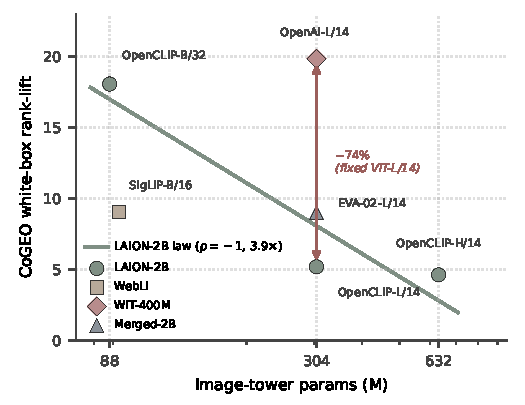
\includegraphics[width=\columnwidth]{figures/fig_capacity_scaling.pdf}
\caption{Retriever capacity compresses the manipulable band. CoGEO white-box mean rank-lift versus image-tower parameter count (log scale, $\eps=16/255$, $224\times224$): within the corpus-controlled LAION-2B family the band contracts monotonically with capacity ($18.07\to5.18\to4.61$, Spearman $\rho=-1.0$, $\approx3.9\times$); a larger or cleaner pretraining corpus compresses it further at fixed capacity ($-74\%$ from OpenAI WIT-400M to LAION-2B at ViT-L/14). The all-six correlation is a non-significant $\rho=-0.64$.}
\label{fig:extval}
\end{figure}

\paragraph{External validity beyond ESCI/OpenAI} The same four-method ordering is preserved on Food-101 (Fig.~\ref{fig:results}f), so the ceiling and ordering above are properties of the attack family rather than artifacts of the ESCI/OpenAI pairing.

\subsection{The transfer axis: significant but bounded held-out rank-lift}
\label{sec:analysis:transfer}

AE-CoGEO is the first query-free, anchor-decoupled cross-encoder probe whose role is to \emph{measure} this transfer axis as a calibrated instrument, not to mount a leaderboard or SOTA attack. One perturbation optimized against the four-encoder source consensus is scored, without re-attack, on four held-out encoders absent from the source set, against a single-encoder CoGEO reference arm (optimized against OpenAI ViT-L/14 alone) transferred to the same encoders. The only difference between arms is the source set ($n=498$ paired ESCI pairs, $\eps=16/255$), isolating the transfer mechanism (\S\ref{sec:method:aecogeo}).

\begin{table}[htbp]
\centering
\caption{Held-out-encoder transfer rank-lift (mean positions gained, $n = 498$, $\eps = 16/255$). The single-encoder arm transfers a CoGEO perturbation optimized against OpenAI ViT-L/14 alone; the AE-CoGEO arm transfers one optimized against the four-encoder source consensus (\S\ref{sec:method:aecogeo}); no held-out encoder appears in the source set. $p$: one-sided paired Wilcoxon of AE-CoGEO over the single-encoder baseline. $^{\dagger}$LAION-2B-pretrained.}
\label{tab:transfer}
\small
\setlength{\tabcolsep}{4pt}
\begin{tabular}{lrrr}
\toprule
Held-out encoder & Single-enc & AE-CoGEO & $p$ \\
\midrule
OpenCLIP-L/14$^{\dagger}$ & 1.04 & \textbf{3.29} & $7 \times 10^{-5}$ \\
OpenCLIP-H/14$^{\dagger}$ & 3.63 & \textbf{5.85} & $< 10^{-3}$ \\
OpenCLIP-B/32$^{\dagger}$ & 7.28 & \textbf{8.60} & $0.016$ \\
SigLIP ViT-B/16           & 3.07 & \textbf{4.80} & $1.3 \times 10^{-3}$ \\
\midrule
\multicolumn{4}{@{}l}{\footnotesize Strongest-source white-box: $\mathbf{18.47}$ (transfer ceiling)}\\
\bottomrule
\end{tabular}
\end{table}

\paragraph{Consensus transfer is real and statistically significant} The consensus lifts mean held-out rank-lift over the single-encoder baseline on all four unseen encoders, each gain significant at the per-comparison level (one-sided paired Wilcoxon, $p\in[7\times10^{-5},\,0.016]$; Table~\ref{tab:transfer}, Fig.~\ref{fig:results}c). A residual threat thus exists: an attacker ensembling public CLIP encoders measurably moves a retriever it never optimized against.

\paragraph{The transfer threat stays far below the white-box ceiling, across paradigms} The same source-consensus perturbation evaluated white-box on its strongest source encoder reaches the transfer ceiling of $18.47$ (Table~\ref{tab:transfer}), two-to-six times the transferred $3.3$--$8.6$. Scored without re-attack on a fused-encoder BLIP image--text reranker~\cite{li2022blip} that shares no encoder or objective with the source set ($n=500$), it reaches only $7.52$, still inside the held-out band (Fig.~\ref{fig:bounded}a): the deflation of \S\ref{sec:experiments} survives the strongest transfer attack \emph{and} a change of retrieval paradigm, and the training-free detector flags it (AUROC $0.990$).

\paragraph{Consensus transfer scales monotonically with the source-encoder count} Growing the source set from one to four public CLIP encoders raises the pooled held-out transfer monotonically ($3.76 \to 5.64$, Spearman $\rho = 1.0$; Fig.~\ref{fig:results}a), so AE-CoGEO is a genuine ensemble-transfer instrument with a measurable scaling law.

\subsection{Anchor-source robustness}
\label{sec:analysis:anchor}

\begin{figure}[tb]
\centering
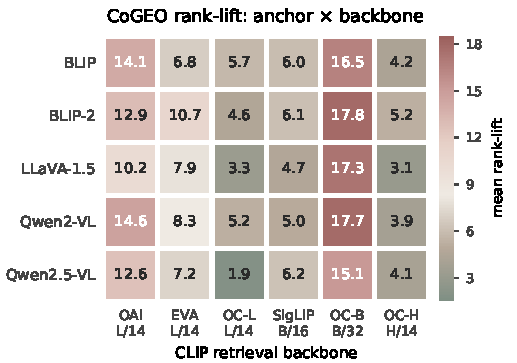
\includegraphics[width=0.92\columnwidth]{figures/fig_anchor_heatmap.pdf}
\caption{CoGEO mean rank-lift across $5$ VLM caption anchors (rows) $\times$ $6$ CLIP backbones (columns) on the $491$-ASIN ESCI manifest ($\eps=16/255$): OAI~L/14, EVA (EVA-02 L/14), OC-L (OpenCLIP L/14), SigLIP (B/16), OC-B (OpenCLIP B/32), OC-H (OpenCLIP H/14). Column means span $4.1$--$16.9$ but row means only $7.7$--$9.6$: the retriever, not the anchor captioner, explains the bulk of the spread---the signature of an anchor-decoupled protocol.}
\label{fig:anchorbb}
\end{figure}

Because the protocol requires only that the anchor be a function of $x_p$, we re-run CoGEO against the same six retrievers with five VLM captioners, giving the $5 \times 6$ rank-lift matrix of Fig.~\ref{fig:anchorbb}. Two facts hold: the retriever dominates the anchor (per-backbone column means span $4.1$--$16.9$, versus only $7.7$--$9.6$ across the five anchor captioners), and no captioner is uniformly best (within-column gap under $5$ positions). Both confirm \eqref{eq:invariant}: any function of $x_p$ alone is an admissible anchor, so the protocol surfaces an encoder-side property rather than a captioner artifact.

\subsection{Bounded under stress: transfer, defense, and scale-up}
\label{sec:analysis:summary}

The remaining robustness, transfer, and defense experiments are consolidated into one display, Figure~\ref{fig:bounded} (full per-pair data and per-experiment construction in the released artifact). Three messages emerge.

\paragraph{The white-box rank-lift is a genuine ceiling} Every out-of-source transfer probe --- a four-encoder AE-CoGEO consensus, a BLIP fused-encoder reranker, a BLIP-2 Q-Former, and a late-interaction MaxSim matcher --- stays far below it (Fig.~\ref{fig:bounded}a), so the deflation survives a change of encoder, of retrieval paradigm, and of matching mechanism. A fifth, diffusion-prior attack family lands mid-pack ($13.18$, below CoGEO's $15.60$ on the matched $n{=}500$ five-family panel; Table~\ref{tab:statsextra}), so CoGEO holds the top point estimate across five families --- though their $95\%$ CIs overlap and ranks $2$--$4$ are sample-dependent (Co-Attack $12.82$ vs $5.77$ at $560$ pairs); the per-pair distributions are strongly right-skewed for all five (Fig.~\ref{fig:distribution}).

\paragraph{The bounded operator is defender-containable, and heterogeneity is not an exploitable handle} A training-free Laplacian detector flags all four families and the AE-CoGEO transfer perturbation at AUROC $\geq0.99$, generalizing across families and to a held-out domain, degrading only as the budget shrinks (Table~\ref{tab:statsextra}); small-budget input purification removes most of the residual lift (further reduced under cohort-aware oracle allocation), and even a matched adaptive attacker stays far below the ceiling (Fig.~\ref{fig:bounded}b). A cohort-adaptive-budget (CAB) attacker redistributing a matched mean budget toward cheaper-to-move cohorts \emph{under-performs} a uniform budget ($13.0$ vs $15.6$), so heterogeneity is a diagnostic, not a handle; no tested budget is both potent and detector-evasive.

\paragraph{The findings are not small-sample artifacts} Rebuilding a label-balanced ESCI sample three times larger ($1{,}430$ pairs) sharpens the per-cohort gradient and the mean-shift, not per-pair directional dominance (Fig.~\ref{fig:bounded}c). Across all four families at this scale the mean rank-lift ordering is CoGEO $41.26 >$ Co-Attack $34.05 \approx$ PGD-bare $33.38 >$ AdvCLIP $26.16$: CoGEO has the highest mean, with Co-Attack and PGD-bare near-tied at ranks $2$--$3$. The CoGEO$-$PGD-bare lead is $+7.89$ (bootstrap 95\% CI $[2.0,13.6]$, excluding zero) yet the paired directional Wilcoxon stays non-significant ($p{=}0.78$), so the mean advantage is tail-driven; both anchor attacks nonetheless rise strictly ($E\!<\!S\!<\!C\!<\!I$), resolving rather than reproducing the small-sample $560$-pair Complement-peak ordering ($E\!<\!S\!<\!I\!<\!C$, Table~\ref{tab:cohort}), the Exact reversal vanishing. Two directional controls reinforce this: Gaussian noise at the same budget is stealthier than every attack (SSIM $0.854$) yet yields $\approx0$ rank-lift, and the same attack scored at the larger $800^2$ input is more stealthy (SSIM $\geq0.98$) but loses essentially all lift, making resolution a third trade-off axis (C3; both shown in Fig.~\ref{fig:results}e).

\begin{figure}[t]
\centering
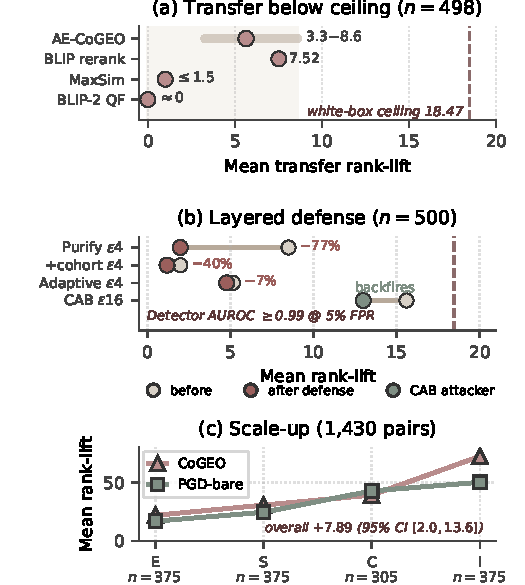
\includegraphics[width=\columnwidth]{figures/fig_bounded_defense.pdf}
\caption{Consolidated robustness, transfer, and defense evidence (rank-lift vs.\ the $18.47$ white-box ceiling; panel (c) is an independent $1{,}430$-pair scale-up with its own axis). \textbf{(a)} Out-of-source transfer: the AE-CoGEO four-encoder consensus ($3.3$--$8.6$), a BLIP fused-encoder reranker ($7.52$), a late-interaction MaxSim probe ($\leq1.5$), and a BLIP-2 Q-Former ($\approx0$) all sit far below the ceiling. \textbf{(b)} Layered defense at $\eps{=}4/255$ (before~$\to$~after): input purification ($8.50\to1.98$, $-77\%$), cohort-aware oracle ($-40\%$ further), and a matched adaptive attacker ($5.15\to4.77$); at $\eps{=}16/255$ a cohort-adaptive-budget attacker under-performs uniform ($13.0$ vs $15.6$) and a training-free detector flags every family at AUROC $\geq0.99$. \textbf{(c)} The $3\times$ scale-up sharpens the per-cohort gradient into a strictly monotone $E\!<\!S\!<\!C\!<\!I$ for both load-bearing attacks (CoGEO$-$PGD $+7.89$, 95\% CI $[2.0,13.6]$). Values match \S\ref{sec:analysis:summary}.}
\label{fig:bounded}
\end{figure}

\begin{table}[t]
\centering
\caption{Two further checks (OpenAI ViT-L/14, $n{=}500$). \emph{Top}: per-pair rank-lift for five white-box families at $\eps{=}16/255$; all are right-skewed (median $\approx1$) with CoGEO the top point estimate (overlapping CIs). \emph{Bottom}: training-free Laplacian-detector AUROC by budget, $\geq0.99$ at $\eps{=}16/255$ and degrading only as the budget shrinks.}
\label{tab:statsextra}
\footnotesize
\setlength{\tabcolsep}{4.2pt}
\begin{tabular}{@{}lrccrr@{}}
\toprule
\multicolumn{6}{@{}l}{\textbf{Five attack families (white-box), per-pair rank-lift}}\\
Family & Mean & 95\% CI & Med. & \%\,$\le0$ & Max\\
\midrule
\textbf{CoGEO} & \textbf{15.60} & [10.9, 20.3] & 1.0 & 47.0 & 354\\
PGD-bare & 13.58 & [8.3, 18.8] & 1.0 & 48.2 & 390\\
Diffusion-prior & 13.18 & [8.5, 17.9] & 1.0 & 48.8 & 388\\
Co-Attack & 12.82 & [8.2, 17.5] & 1.0 & 48.0 & 348\\
AdvCLIP & 5.06 & [1.8, 8.4] & 0.0 & 63.4 & 281\\
\midrule
\multicolumn{6}{@{}l}{\textbf{Training-free detector AUROC by budget}}\\
$\eps{=}16/255$ & \multicolumn{2}{l}{0.99--1.00} & \multicolumn{3}{l@{}}{$\eps{=}8/255$:\ 0.957--0.970}\\
$\eps{=}4/255$ & \multicolumn{2}{l}{0.852--0.889} & \multicolumn{3}{l@{}}{Food-101:\ 1.00}\\
\bottomrule
\end{tabular}
\end{table}

\begin{figure}[t]
\centering
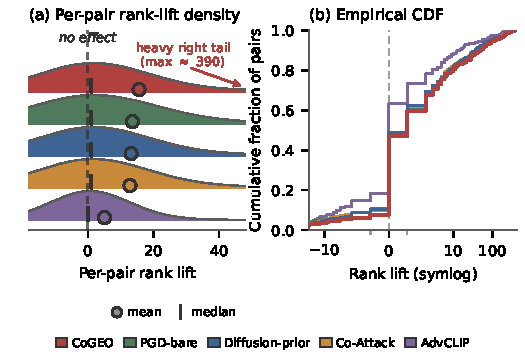
\includegraphics[width=\columnwidth]{figures/fig_distribution}
\caption{Per-pair rank-lift distribution for the five white-box attack families (OpenAI ViT-L/14, $n{=}500$ each, $\eps{=}16/255$). \textbf{(a)} Ridgeline densities: every family is strongly right-skewed---the typical pair barely moves (median $\approx1$; dashed ``no effect'' line) while a heavy right tail (up to $\approx390$) lifts the mean (open circles). \textbf{(b)} Empirical CDF on a symlog axis: the lower/further-right a curve, the heavier its tail; CoGEO is heaviest, AdvCLIP lightest, with $\geq47\%$ of pairs unaffected ($\le0$) for every family. The headline mean thus summarises a sparse, skewed effect, not a uniform shift.}
\label{fig:distribution}
\end{figure}

\section{Limitations}
\label{sec:limitations}

The empirical scope is intentionally narrow. \textbf{Architecture.} Our six retrievers~\cite{radford2021clip,cherti2023reproducible,fang2023eva02,zhai2023siglip} span two pretraining corpora and three scales but share the CLIP dual-encoder paradigm; \S\ref{sec:analysis:transfer} measures transfer to a BLIP fused-encoder reranker~\cite{li2022blip}, which retains bounded positive transfer (mean rank-lift $7.52$, within the $3.3$--$8.6$ held-out-CLIP band), while a BLIP-2 Q-Former reranker~\cite{li2023blip2} (released artifact) shows no positive transfer. A training-free late-interaction (MaxSim) probe shows the same bounded behavior; fully trained late-interaction and learned-hashing retrievers are left to future work. Within each backbone the encoder pair is both optimization target and evaluation embedder, so headline numbers are a white-box upper bound. \textbf{Resolution and budget.} Headline rankings use $224 \times 224$ at $\eps = 16/255$; the released artifact reports two crossovers ($800 \times 800$: CoGEO turns marginally negative, overtaken by PGD-bare; $\eps = 4/255$: PGD-bare slightly exceeds CoGEO), so dominance requires a budget large enough to amortize CoGEO's auxiliary objectives. \textbf{Attack and benchmark scope.} The four-attack shortlist~\cite{madry2018pgd,zhou2023advclip,zhang2022coattack,moosavidezfooli2017uap} covers per-image gradient, universal-patch, and cross-modal families; evolutionary search is unmeasured. Crucially, the per-cohort human-relevance findings rest on ESCI's graded labels~\cite{reddy2022esci} alone: the Food-101 cohorts are retriever-induced (CLIP-text-similarity quartiles), not human relevance, so they probe robustness rather than substitute for graded evidence. A survey of public alternatives found none simultaneously offering a second product domain, multi-level human relevance, and usable images, so this evidence stays single-domain. \textbf{Anchor independence.} The invariant of \eqref{eq:invariant} closes the immediate optimization-anchor/eval-query loop but not the deeper seller-ecosystem/training-corpus loop; the VLM-anchor ablation (released artifact) bounds within-anchor variation by under $5$ rank positions across five captioners and six backbones, narrowing the self-loop critique rather than erasing the per-cohort findings.

\section{Conclusion}
\label{sec:conclusion}

\paragraph{Findings} We recalibrate visual GEO into something a defender can act on. Within the anchor-decoupled protocol, a four-way comparison on Amazon ESCI~\cite{radford2021clip,reddy2022esci} across six retrievers at $\eps = 16/255$ replaces optimistic self-loop scores with an honest measurement: per-image gradient optimization significantly outperforms universal-patch and cross-modal baselines (Wilcoxon $p \leq 1.1 \times 10^{-4}$), yet the per-cohort lens exposes an Exact-cohort statistical match and a monotonic stealth/lift trade-off.

\paragraph{Contribution 1: an honest recalibration} At its core is an evaluation methodology: an anchor$\perp$query invariant, a pre-flight retriever-discrimination gate, and a per-cohort decomposition over the four ESCI relevance classes~\cite{reddy2022esci}. Through the protocol, transfer, and detection results, visual GEO is not a uniform invisible threat but a cohort-specific, white-box-bounded, transfer-limited, detectable ($\mathrm{AUROC} \geq 0.99$ at $\eps{=}16/255$ on a balanced benchmark) operator. Detectability and efficacy rise and fall together, so no tested budget makes visual GEO simultaneously effective and evasive (Fig.~\ref{fig:bounded}): a cheap input-purification knob narrows the small-budget gap, and the per-cohort heterogeneity, though not an exploitable handle, is defender-actionable through an oracle cohort allocation, with a practical cohort router left to future work.

\paragraph{Contribution 2: AE-CoGEO, a new cross-encoder transfer attack} To our knowledge the first of its kind for visual GEO (\S\ref{sec:method:aecogeo},~\ref{sec:analysis:transfer}), it outperforms the single-encoder transfer baseline on all four held-out encoders by a small but consistent margin ($+1.3$ to $+2.3$ positions), with a monotone source-count scaling law (Spearman $\rho = 1.0$), yet its transfer stays far below the same source-consensus white-box ceiling ($3.3$--$8.6$ versus $18.47$), sharpening rather than overturning the recalibration.

\paragraph{Future work} Future visual-GEO claims should report stealth and rank-lift jointly at the retriever's native input size; since the $1{,}430$-pair scale-up already sharpens the per-cohort findings into strict monotonicity, the principal remaining gap is breadth across product domains, not sample size. The protocol and both attacks ship anonymously as \textsc{HonestVGEO} (\url{https://anonymous.4open.science/r/honestvgeo-F663}).

\paragraph{Ethics and responsible disclosure} We release AE-CoGEO and the protocol as a defensive recalibration instrument, not an operational attack, shipping the training-free detector and the input-purification knob alongside the attack. Because the evaluation runs on the public Amazon ESCI research benchmark~\cite{reddy2022esci} rather than any live storefront, the work targets no specific operator; we nonetheless adopt a responsible-disclosure posture and release the defense and the attack together, so that publication strengthens auditing rather than enabling undetected abuse.


% compress reference-list spacing the standard way (IEEEbibitemsep is not a length register in this IEEEtran build and prints stray text)
\let\oldthebibliography\thebibliography
\renewcommand{\thebibliography}[1]{%
  \oldthebibliography{#1}%
  \setlength{\itemsep}{-0.55ex}%
  \setlength{\parsep}{0pt}}
{\footnotesize
\bibliographystyle{IEEEtran}
\bibliography{references}}

\end{document}
